\documentclass[14pt,a4paper,report]{report}
\usepackage[a4paper, mag=1000, left=2.5cm, right=1cm, top=2cm, bottom=2cm, headsep=0.7cm, footskip=1cm]{geometry}
\usepackage[utf8]{inputenc}
\usepackage[english,russian]{babel}
\usepackage{indentfirst}
\usepackage[dvipsnames]{xcolor}
\usepackage[colorlinks]{hyperref}
\usepackage{listings} 
\usepackage{fancyhdr}
\usepackage{caption}
\usepackage{amsmath}
\usepackage{latexsym}
\usepackage{graphicx}
\usepackage{amsmath}
\usepackage{booktabs}
\usepackage{array}
\hypersetup{
	colorlinks = true,
	linkcolor  = black
}

\usepackage{titlesec}
\titleformat{\chapter}
{\Large\bfseries} % format
{}                % label
{0pt}             % sep
{\huge}           % before-code


\DeclareCaptionFont{white}{\color{white}} 

% Listing description
\usepackage{listings} 
\DeclareCaptionFormat{listing}{\colorbox{gray}{\parbox{\textwidth}{#1#2#3}}}
\captionsetup[lstlisting]{format=listing,labelfont=white,textfont=white}
\lstset{ 
	% Listing settings
	inputencoding = utf8,			
	extendedchars = \true, 
	keepspaces = true, 			  	 % Поддержка кириллицы и пробелов в комментариях
	language = Matlab,            	 	 % Язык программирования (для подсветки)
	basicstyle = \small\sffamily, 	 % Размер и начертание шрифта для подсветки кода
	numbers = left,               	 % Где поставить нумерацию строк (слева\справа)
	numberstyle = \tiny,          	 % Размер шрифта для номеров строк
	stepnumber = 1,               	 % Размер шага между двумя номерами строк
	numbersep = 5pt,              	 % Как далеко отстоят номера строк от подсвечиваемого кода
	backgroundcolor = \color{white}, % Цвет фона подсветки - используем \usepackage{color}
	showspaces = false,           	 % Показывать или нет пробелы специальными отступами
	showstringspaces = false,    	 % Показывать или нет пробелы в строках
	showtabs = false,           	 % Показывать или нет табуляцию в строках
	frame = single,              	 % Рисовать рамку вокруг кода
	tabsize = 2,                  	 % Размер табуляции по умолчанию равен 2 пробелам
	captionpos = t,             	 % Позиция заголовка вверху [t] или внизу [b] 
	breaklines = true,           	 % Автоматически переносить строки (да\нет)
	breakatwhitespace = false,   	 % Переносить строки только если есть пробел
	escapeinside = {\%*}{*)}      	 % Если нужно добавить комментарии в коде
}

\begin{document}

\def\contentsname{Содержание}

% Titlepage
\begin{titlepage}
	\begin{center}
		\textsc{Санкт-Петербургский Политехнический 
			Университет Петра Великого\\[5mm]
			Кафедра компьютерных систем и программных технологий}
		
		\vfill
		
		\textbf{Отчёт по лабораторной работе №2\\[3mm]
			Курс: «Методы оптимизации и принятия решений»\\[3mm]
			Тема: «Анализ GERT-сети»\\[35mm]
			}
	\end{center}
	
	\hfill
	\begin{minipage}{.5\textwidth}
		Выполнил студент:\\[2mm] 
		Волкова Мария Дмитриевна\\
		Группа: 13541/2\\[5mm]
		
		Проверил:\\[2mm] 
		Сиднев Александр Георгиевич
	\end{minipage}
	\vfill
	\begin{center}
		Санкт-Петербург\\ \the\year\ г.
	\end{center}
\end{titlepage}

% Contents
\tableofcontents
\clearpage

\chapter{Лабораторная работа №2}

\section{Задание}

\begin{figure}[h!]
	\centering
	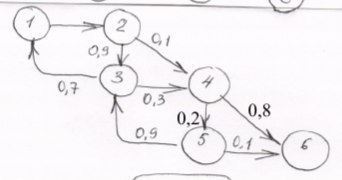
\includegraphics[scale = 1.5]{images/00.jpeg}
	\caption{Исходный граф системы}
	\label{image:0}
\end{figure}

\subsubsection{Часть 1}

Каждой дуге ($ij$) поставлены в соответствие следующие данные:

\begin{itemize}
	\item закон распределения времени выполнения работы (будем считать его нормальным);
	\item параметры закона распределения; (математическое ожидание $M$ и дисперсия $D$).
	\item вероятность $P_{ij}$ выполнения работы, показанная на графе.
\end{itemize}

Необходимо найти:

\begin{itemize}
	\item вероятность выхода в завершающий узел графа (для всех вариантов узел 6);
	\item математическое ожидание;
	\item дисперсию времени выхода процесса в завершающий узел графа;
		\item начальные моменты первых 10 порядков.
\end{itemize}

В отчете перечислить все петли всех порядков, обнаруженные на графе, выписать уравнение Мейсона, получить решение для $W_E(s)$ и найти требуемые параметры.

\subsubsection{Часть 2}

Решить задачу используя методику анализа потокового графа, основанную на обработке матрицы передач (Branch Transmittance Matrix).

\clearpage

\section{Ход работы}

\subsection{Построение замкнутой GERT-сети}

Чтобы определить эквивалентную W-функцию для анализируемой GERT-сети, необходимо замкнуть сеть дугой, исходящей из узла 6 в узел 1:

\begin{figure}[h!]
	\centering
	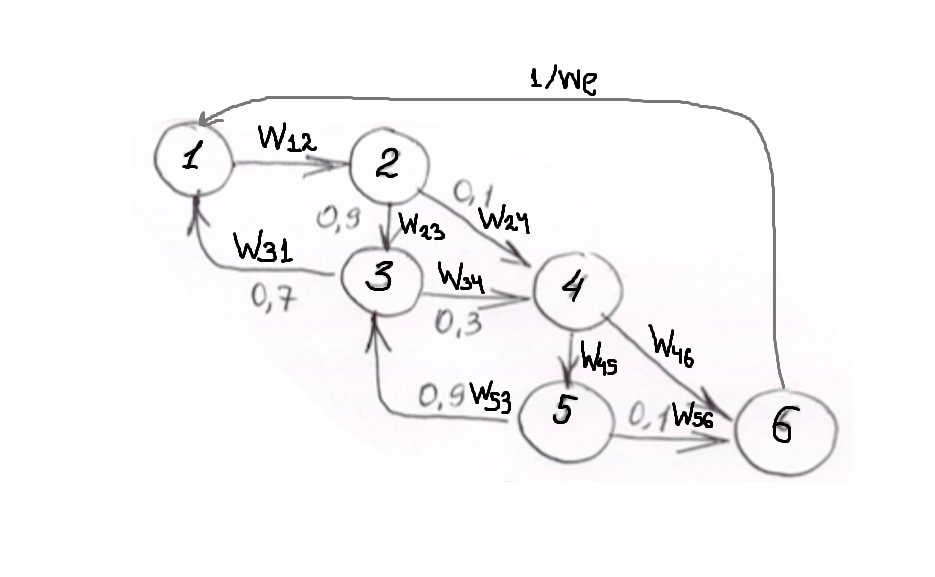
\includegraphics[scale = 0.65]{images/1.png}
	\caption{Замкнутая GERT-сеть}
	\label{image:1}
\end{figure}

\subsection{Построение W-функции}

Найдем W-функции для дуг GERT-сети из производящей функции моментов треугольного распределения и запишем это в таблицу:
$$ MGF = (\frac{2(e^{\frac{sb}{2}}-e^{\frac{sa}{2}})}{(b-a)s})^2 $$
$$ W = P * MGF  $$
\begin{table}[h!]
	\center
	\bgroup
	\def\arraystretch{1}
	\begin{tabular}{ | m{1.5cm} | m{1.5cm} | m{2.0cm} | m{1.0cm} | m{1.0cm} | m{5.0cm} | }
		\hline
		Начало & Конец & Вероятность & M & D & W-функция \\ \hline
		1 	&  2 	& 1 			& 38 	& 16 	& $\frac{0.00192367 (e^{7.6 s} - 1 e^{30.4 s})^2}{s^2}$ \\ \hline
		2	& 3 	& 0.9 		& 19 	& 9 		& $\frac{0.00692521 (e^{3.8 s} - 1 e^{15.2 s})^2}{s^2}$ \\ \hline
		2 	& 4 	& 0.1  		& 32 	& 16 	& $\frac{0.000271267 (e^{6.4 s} - 1 e^{25.6 s})^2}{s^2}$ \\ \hline
		3 	& 1 	& 0.7 		& 33 	& 16 	& $\frac{0.00178553 (e^{6.6 s} - 1 e^{26.4 s})^2}{s^2}$ \\ \hline
		3 	& 4 	& 0.3 		& 20 	& 9 		& $\frac{0.00208333 (e^{4 s} - 1 e^{16 s})^2}{s^2}$ \\ \hline
		4 	& 5 	& 0.2 			& 28 	& 16 	& $\frac{0.000708617 (e^{5.6 s} - 1 e^{22.4 s})^2}{s^2}$ \\ \hline
		4 	& 6 	& 0.8 			& 30 	& 16 	& $\frac{0.00246914 (e^{6 s} - 1 e^{24 s})^2}{s^2}$ \\ \hline
		5 	& 3 	& 0.9 		& 37 	& 16 	& $\frac{0.00182615 (e^{7.4 s} - 1 e^{29.6 s})^2}{s^2}$ \\ \hline
		5 	& 6 	& 0.1 		& 43 	& 25 	& $\frac{0.000150231 (e^{8.6 s} - 1 e^{34.4 s})^2}{s^2}$ \\ \hline
	\end{tabular}
	\egroup
\end{table}

\subsection{Построение уравнения Мейсона}

Петли первого порядка:

$W_{12}\cdot W_{23}\cdot W_{31}$

$W_{34}\cdot W_{45}\cdot W_{53}$

$W_{12}\cdot W_{24}\cdot W_{45}\cdot W_{53}\cdot W_{31}$

$W_{12}\cdot W_{24}\cdot W_{46}\cdot \frac{1}{W_E}$

$W_{12}\cdot W_{24}\cdot W_{45}\cdot W_{56}\cdot \frac{1}{W_E}$

$W_{12}\cdot W_{23}\cdot W_{34}\cdot W_{46}\cdot \frac{1}{W_E}$

$W_{12}\cdot W_{23}\cdot W_{34}\cdot W_{45}\cdot W_{56}\cdot \frac{1}{W_E}$

Петлей второго порядка на графе нет.

Таким образом уравнение Мейсона будет иметь следующий вид:

$H=1 - W_{12}W_{23}W_{31} 
- W_{34}W_{45}W_{53} 
- W_{12}W_{24}W_{45}W_{53}W_{31} 
- W_{12}W_{24}W_{46}\frac{1}{W_E} 
- W_{12}W_{24}W_{45}W_{56}\frac{1}{W_E} 
- W_{12}W_{23}W_{34}W_{36}\frac{1}{W_E} 
- W_{12}W_{23}W_{34}W_{45}W_{56}\frac{1}{W_E}$\\

Получаем эквивалентную W-функцию:

$W_E(s)=- \frac{W_{12}W_{24}W_{46} 
+ W_{12}W_{23}W_{34}W_{45}W_{56}
+ W_{12}W_{23}W_{34}W_{46}
+ W_{12}W_{24}W_{45}W_{56}}
{W_{12}W_{23}W_{31} +W_{12}W_{24}W_{45}W_{53}W_{31}+W_{34}W_{45}W_{53} -1}$\\

\subsection{Рассчет статистических значений}

Расчет математического ожидания ($\mu_{1E}$) и дисперсии ($\sigma_E$) производится по следующим образом:
$$\mu_{1E}=\frac{d M_E(s)}{ds}|s=0$$

$$\mu_{2E}=\frac{d^2 M_E(s)}{ds^2}|s=0$$

$$\sigma^2=\mu_{2E}-\mu_{1E}^2$$

$$ p_E=W_E(0)$$
Далее приведен скрипт для расчета статистических значений в среде MATLAB:
\begin{lstlisting}[language={matlab}, caption={Скрипт Matlab}, basicstyle=\ttfamily]
clc;
format long g;
syms s

P12 = 1;   M12 = 38;
P23 = 0.9; M23 = 19; 
P24 = 0.1; M24 = 32; 
P31 = 0.7; M31 = 33; 
P34 = 0.3; M34 = 20; 
P45 = 0.2;   M45 = 28; 
P46 = 0.8;   M46 = 30; 
P53 = 0.9; M53 = 37; 
P56 = 0.1; M56 = 43; 

a = 0.4;
b = 1.6;

W12 = P12*((2*(exp((s*b*M12)/2)-exp((s*a*M12)/2)))/((b*M12-a*M12)*s))^2;
W46 = P46*((2*(exp((s*b*M46)/2)-exp((s*a*M46)/2)))/((b*M46-a*M46)*s))^2;
W24 = P24*((2*(exp((s*b*M24)/2)-exp((s*a*M24)/2)))/((b*M24-a*M24)*s))^2;
W34 = P34*((2*(exp((s*b*M34)/2)-exp((s*a*M34)/2)))/((b*M34-a*M34)*s))^2;
W45 = P45*((2*(exp((s*b*M45)/2)-exp((s*a*M45)/2)))/((b*M45-a*M45)*s))^2;
W23 = P23*((2*(exp((s*b*M23)/2)-exp((s*a*M23)/2)))/((b*M23-a*M23)*s))^2;
W31 = P31*((2*(exp((s*b*M31)/2)-exp((s*a*M31)/2)))/((b*M31-a*M31)*s))^2;
W53 = P53*((2*(exp((s*b*M53)/2)-exp((s*a*M53)/2)))/((b*M53-a*M53)*s))^2;
W56 = P56*((2*(exp((s*b*M56)/2)-exp((s*a*M56)/2)))/((b*M56-a*M56)*s))^2;

We = -((W12*W23*W34*W45*W56 + W12*W23*W34*W46 + W12*W24*W46 + W12*W24*W45*W56)/(W12*W23*W31 + W34*W45*W53 + W12*W24*W45*W53*W31 - 1));
We = simplify(We);
We0 = limit(We, 's', 0);

% We(0)
% We0 = subs(We, 's', 0);
fprintf('We(0) = %.3f\n', double(We0));

M = We / We0;

m1 = diff(M, 's', 1);
m1 = limit(m1, 's', 0);
fprintf('m1 = %.3f\n', double(m1));

m2 = diff(M, 's', 2);
m2 = limit(m2, 's', 0);
fprintf('m2 = %.3f\n', double(m2));

D = me2 - me1 ^ 2;
fprintf('D = %.3f\n', double(D ));
\end{lstlisting}


Результат вычисления статистических значений:

\begin{lstlisting}[language={matlab}, caption={Matlab скрипт}, basicstyle=\ttfamily]
We(0) = 1.000
m1 = 315.096
m2 = 162883.236
D = 63598.009
\end{lstlisting}

Были получены следующие результаты:
\begin{enumerate}
\item Вероятность выхода в завершающий граф узла 100\%.
\item Математическое ожидание 315.096.
\item Дисперсия времени выхода процесса в завершающий узел графа 63598.009.
\end{enumerate}


\subsection{Часть 2}

Определим матрицу Q:
\begin{equation*}
Q = 
 \begin{pmatrix}
  0 & q_{12} & 0 & 0 & 0 & 0 \\
  0 & 0 & q_{23} & q_{24} & 0 & 0 \\ 
  q_{31} & 0 & 0 & q_{34} & 0 & 0 \\ 
  0 & 0 & 0 & 0 & q_{45} & q_{46} \\ 
  0 & 0 & q_{53} & 0 & 0 & q_{56} \\ 
  w_{61} & 0 & 0 & 0 & 0 & 0 
 \end{pmatrix}
\end{equation*}
Определим матрицу коэффициентов $A=I_6-Q^T$.
\begin{equation*}
A = 
 \begin{pmatrix}
    1&       0&    -q_{31}&    0&    0& -w_{61}\\
 -q_{12}& 1 & 0&    0&       0&    0\\
    0&    -q_{23}&    1&    0&       -q_{53}&    0\\
    0&       -q_{24}& -q_{34}&    1&       0&    0\\
    0&       0&    0& -q_{45}& 1 &    0\\
    0&       0&    0&    -q_{46}&    -q_{56}&    1
 \end{pmatrix}
\end{equation*}
Находим 
\begin{equation*}
det(A)
\end{equation*}
далее
\begin{equation*}
\frac{\partial det(A)}{\partial w_{61}}
\end{equation*}
\begin{equation*}
det(A | w_{61}=0)
\end{equation*}
Далее можно вывести $W_E(S)$ с помощью формулы:
\begin{equation*}
W_E(S)=-\frac{\frac{\partial det(A)}{\partial w_{61}}}{det(A | w_{61}=0)}
\end{equation*}
Для расчетов, был написан matlab скрипт.
\begin{lstlisting}[language={matlab}, caption={Matlab скрипт}, basicstyle=\ttfamily]
close all; clc;
format long g;

P12 = 1;   M12 = 38;
P23 = 0.9; M23 = 19; 
P24 = 0.1; M24 = 32; 
P31 = 0.7; M31 = 33; 
P34 = 0.3; M34 = 20; 
P45 = 0.2;   M45 = 28; 
P46 = 0.8;   M46 = 30; 
P53 = 0.9; M53 = 37; 
P56 = 0.1; M56 = 43; 

a = 0.4;
b = 1.6;

syms q12
syms q23
syms q31
syms q24
syms q34
syms q45
syms q53
syms q46
syms q56
syms w61
syms s

Q=[0 q12 0 0 0 0;
   0 0 q23 q24 0 0;
   q31 0 0 q34 0 0;
   0 0 0 0 q45 q46;
   0 0 q53 0 0 q56;
   w61 0 0 0 0 0];

A1 = eye(size(Q,1)) - transpose(Q);

det_A1 = det(A1);
fprintf('det_A1 = ');
disp(det_A1);

det_dw=diff(det_A1, w61);
fprintf('det_dw =  ');
disp(det_dw);

det2_A1=subs(det_A1, w61, 0);
fprintf('det2_A1 =  ');
disp(det2_A1);

We= -det_dw/det2_A1;
fprintf('We =  ');
disp(We);

We=subs(We, q12, P12*((2*(exp((s*b*M12)/2)-exp((s*a*M12)/2)))/((b*M12-a*M12)*s))^2);
We=subs(We, q23, P23*((2*(exp((s*b*M23)/2)-exp((s*a*M23)/2)))/((b*M23-a*M23)*s))^2 );
We=subs(We, q31, P31*((2*(exp((s*b*M31)/2)-exp((s*a*M31)/2)))/((b*M31-a*M31)*s))^2);
We=subs(We, q24, P24*((2*(exp((s*b*M24)/2)-exp((s*a*M24)/2)))/((b*M24-a*M24)*s))^2);
We=subs(We, q34, P34*((2*(exp((s*b*M34)/2)-exp((s*a*M34)/2)))/((b*M34-a*M34)*s))^2);
We=subs(We, q45, P45*((2*(exp((s*b*M45)/2)-exp((s*a*M45)/2)))/((b*M45-a*M45)*s))^2);
We=subs(We, q53, P53*((2*(exp((s*b*M53)/2)-exp((s*a*M53)/2)))/((b*M53-a*M53)*s))^2);
We=subs(We, q46, P46*((2*(exp((s*b*M46)/2)-exp((s*a*M46)/2)))/((b*M46-a*M46)*s))^2);
We=subs(We, q56, P56*((2*(exp((s*b*M56)/2)-exp((s*a*M56)/2)))/((b*M56-a*M56)*s))^2);

We = simplify(We);
We0 = limit(We, 's', 0);
fprintf('We(0) = %.3f\n', double(We0));

M = We/We0;
 
m1 = diff(M, 's',1);
m1 = limit(m1, 's', 0);
fprintf('me1 = %.3f\n', double(m1));

m2 = diff(M, 's',2);
m2 = limit(m2, 's', 0);
fprintf('me2 = %.3f\n', double(m2));

D = m2 - (m1)^2;
fprintf('D = %.3f\n', double(D));
\end{lstlisting}


\begin{lstlisting}[language={matlab}, caption={Результат}, basicstyle=\ttfamily]
det_A1 = 1 - q34*q45*q53 - q12*q24*q46*w61 - q12*q24*q31*q45*q53 - q12*q23*q34*q46*w61 - q12*q24*q45*q56*w61 - q12*q23*q34*q45*q56*w61 - q12*q23*q31
 
det_dw =  - q12*q24*q46 - q12*q23*q34*q46 - q12*q24*q45*q56 - q12*q23*q34*q45*q56
 
det2_A1 =  1 - q34*q45*q53 - q12*q24*q31*q45*q53 - q12*q23*q31
 
We =  -(q12*q24*q46 + q12*q23*q34*q46 + q12*q24*q45*q56 + q12*q23*q34*q45*q56)/(q12*q23*q31 + q34*q45*q53 + q12*q24*q31*q45*q53 - 1)
 
We(0) = 1.000
m1 = 315.096
m2 = 162883.236
D = 63598.009
\end{lstlisting}

Были получены следующие результаты:
\begin{enumerate}
\item Вероятность выхода в завершающий граф узла 100\%.
\item Математическое ожидание 315.096.
\item Дисперсия времени выхода процесса в завершающий узел графа 63598.009.
\end{enumerate}

Решив задачу с помощью Branch Transmittance Matrix проверяем, что формула Мейсона, дисперсия, математическое ожидание и вероятность выхода совпадают. 





\section{Вывод}
В ходе данной лабораторной работы были получены навыки работы с вероятностными графами и их обработка с помощью методики GERT. При заданных значениях вероятности, математического ожидания и дисперсии для каждой дуги исходного были выведены W-функции, получена формула Мейсона и рассчитаны математическое ожидание и дисперсия.

Решив задачу с помощью метода анализа потокового графа получили те же значения.
\end{document}